% THIS IS SIGPROC-SP.TEX - VERSION 3.1
% WORKS WITH V3.2SP OF ACM_PROC_ARTICLE-SP.CLS
% APRIL 2009
%
% It is an example file showing how to use the 'acm_proc_article-sp.cls' V3.2SP
% LaTeX2e document class file for Conference Proceedings submissions.
% ----------------------------------------------------------------------------------------------------------------
% This .tex file (and associated .cls V3.2SP) *DOES NOT* produce:
%       1) The Permission Statement
%       2) The Conference (location) Info information
%       3) The Copyright Line with ACM data
%       4) Page numbering
% ---------------------------------------------------------------------------------------------------------------
% It is an example which *does* use the .bib file (from which the .bbl file
% is produced).
% REMEMBER HOWEVER: After having produced the .bbl file,
% and prior to final submission,
% you need to 'insert'  your .bbl file into your source .tex file so as to provide
% ONE 'self-contained' source file.
%
% Questions regarding SIGS should be sent to
% Adrienne Griscti ---> griscti@acm.org
%
% Questions/suggestions regarding the guidelines, .tex and .cls files, etc. to
% Gerald Murray ---> murray@hq.acm.org
%
% For tracking purposes - this is V3.1SP - APRIL 2009

\documentclass{acm_proc_article-sp}

\usepackage{url}
\usepackage{listings} 
% \usepackage{draftwatermark}
% \SetWatermarkText{DRAFT}
% \SetWatermarkScale{5}
% "define" Scala
\lstdefinelanguage{scala}{morekeywords={class,object,trait,extends,with,new,if,while,for,def,val,var,this},
otherkeywords={->,=>},
sensitive=true,
morecomment=[l]{//},
morecomment=[s]{/*}{*/},
morestring=[b]"}
% Default settings for code listings
\lstset{frame=tb,language=scala,aboveskip=3mm,belowskip=3mm,showstringspaces=false,columns=flexible,basicstyle={\small\ttfamily}}

\begin{document}

\title{Rethinking Scientific Analysis Using \linebreak Modern Scalable Systems}
%
% You need the command \numberofauthors to handle the 'placement
% and alignment' of the authors beneath the title.
%
% For aesthetic reasons, we recommend 'three authors at a time'
% i.e. three 'name/affiliation blocks' be placed beneath the title.
%
% NOTE: You are NOT restricted in how many 'rows' of
% "name/affiliations" may appear. We just ask that you restrict
% the number of 'columns' to three.
%
% Because of the available 'opening page real-estate'
% we ask you to refrain from putting more than six authors
% (two rows with three columns) beneath the article title.
% More than six makes the first-page appear very cluttered indeed.
%
% Use the \alignauthor commands to handle the names
% and affiliations for an 'aesthetic maximum' of six authors.
% Add names, affiliations, addresses for
% the seventh etc. author(s) as the argument for the
% \additionalauthors command.
% These 'additional authors' will be output/set for you
% without further effort on your part as the last section in
% the body of your article BEFORE References or any Appendices.

%  in this sample file, there are a *total*
% of EIGHT authors. SIX appear on the 'first-page' (for formatting
% reasons) and the remaining two appear in the \additionalauthors section.
%
\author{}
% You can go ahead and credit any number of authors here,
% e.g. one 'row of three' or two rows (consisting of one row of three
% and a second row of one, two or three).
%
% The command \alignauthor (no curly braces needed) should
% precede each author name, affiliation/snail-mail address and
% e-mail address. Additionally, tag each line of
% affiliation/address with \affaddr, and tag the
% e-mail address with \email.
%
% 1st. author% There's nothing stopping you putting the seventh, eighth, etc.
% author on the opening page (as the 'third row') but we ask,
% for aesthetic reasons that you place these 'additional authors'
% in the \additional authors block, viz.

% Just remember to make sure that the TOTAL number of authors
% is the number that will appear on the first page PLUS the
% number that will appear in the \additionalauthors section.

\maketitle

\begin{abstract}
Revolutions in data acquisition are drastically changing how science conducts experiments. For
example, ``next-\linebreak generation'' sequencing technologies have driven exponential growth in
the volume of genomic data, and similar trends impact many fields which rely on imaging, such as
astronomy and neuroscience. Although there have been early attempts to use MapReduce systems
to accelerate the processing of these datasets, they have conceded efficiency in favor of using legacy
storage formats and software.

Since the amount of scientific data that is being captured is increasing exponentially, we have a good
opportunity to rethink how we process and store these datasets. In this paper, we introduce a set of
principles for implementing scientific analyses efficiently using commodity ``big data'' systems. We
motivate these principles with an example genomics pipeline which leverages open-source MapReduce
and columnar storage techniques to achieve a $>50\times$ speedup over traditional genomics systems,
at half the cost.
\end{abstract}

% A category with the (minimum) three required fields
\category{L.4.1}{Applied Computing}{Life and medical sciences}[Computational biology]
\category{H.1.3.2}{Information Systems}{Data management systems}[Database management
system engines, parallel and distributed DBMSs]
\category{E.3.2}{Software and its Engineering}{Software creation and management}[Software
Development Process Management]

\terms{Design}

\keywords{Analytics, MapReduce, Genomics, Scientific Computing}

\section{Introduction}
\label{sec:introduction}

With major improvements in scientific data acquisition techniques, data storage and processing have
become major problems for scientists~\cite{schadt10, cunningham14}. In fields like
neuroscience~\cite{freeman14} and genomics~\cite{stein10}, scientists routinely perform experiments
that use terabytes~(TB) to petabytes~(PB) of data. While traditional scientific computing platforms are
optimized for fast linear algebra, many emerging domains make heavy use of statistical learning
techniques coupled with user defined operations on top of semistructured data. This move towards
statistical techniques has been driven by the increase in the amount of data available to scientists, as
well as the rise of statistical systems which are accessible to non-experts, such as
\texttt{Scikit-learn}~\cite{pedregosa11} and \texttt{MLI}~\cite{sparks13}.

While the increase in the amount of scientific data available is a boon for scientists, it puts significant
stress on existing tool chains. Using the current ``best practice'' genomics software~\cite{auwera13}, it
takes approximately 120 hours to process a single, high-quality human genome using a single,
beefy node~\cite{talwalkar14}. To address these challenges, scientists have started to apply computer
systems techniques such as MapReduce~\cite{mckenna10, schatz09, langmead09} and columnar
storage~\cite{fritz11} to custom scientific compute/storage systems. While these systems have improved
the analysis cost and performance, they incur significant overheads due to constraints of the legacy
formats and codebases that they use.

Since the amount of scientific data being generated is growing so quickly, we cannot afford to be
saddled by legacy software and formats. New scientific projects such as the ``100K for UK,'' which aims
to sequence the genomes of 100,000 individuals in the United Kingdom~(UK, \cite{uk100k}) will
generate three to four orders of magnitude more data than prior ``massive'' projects such as the 1000
Genomes Project~\cite{siva08}. While it is important to still be able to use data stored in legacy formats,
the massive amount of \emph{new} data provides us with an opportunity to rethink how we compose
our systems. By choosing the correct mix of computing systems, we can provide better performance and
scalability than custom systems, while enhancing the abstractions exposed to scientists.

In this paper, we demonstrate a system built using Apache Avro, Parquet, and Spark~\cite{avro, parquet,
zaharia10}, which achieves a 50$\times$ increase in throughput over the current best practice pipeline
for processing genomic data. In the process of creating this system, we developed a ``narrow waisted''
layering model for building similar scientific analysis systems. This narrow waisted model is inspired by
the OSI model for networked systems~\cite{zimmermann80}. We then demonstrate the generality of this
model by using it to implement a system for processing astronomy images.

A subtle problem with earlier custom scientific processing and storage systems is that characteristics
of the data format on disk would bleed into the computing model. For example, in the current
Sequence/Binary Alignment and Map~(SAM/BAM~\cite{li09}) formats for storing genomic alignments,
constraints about record ordering are required in order to enable specific computing patterns. We
believe that this is an abstraction inversion, which makes it difficult to perform some other access
patterns. In~\S\ref{sec:principles}, we elucidate why this is a significant problem, and then
in~\S\ref{sec:optimizations-scientific-processing}, we then introduce efficient algorithms for supporting
these computational patterns without forcing constraints on the storage layer.

\section{Background}
\label{sec:background}

As our work exists at the intersection of computational science and data management and processing
systems, our architectural approach is informed by recent trends in both areas. The design of large
scale data management has changed dramatically since the landmark papers by Dean and
Ghemawat~\cite{dean04, dean08} which described Google's \texttt{MapReduce} system. Over a
similar timeframe, scientific fields have moved to take advantage of improvements in data acquisition
technologies. For example, since the Human Genome Project finished in 2001~\cite{lander01}, the price
of genomic sequencing has dropped by 10,000$\times$~\cite{nhgri}. This drop in cost has enabled the
capture of petabytes of sequence data, which has enabled significant population-scale genomics
experiments like the 1000 Genomes project~\cite{siva08}, and The Cancer Genome Atlas~(TCGA,
\cite{weinstein13}). These changes are not unique to genomics; indeed, fields such as
neuroscience~\cite{cunningham14} and astronomy~\cite{turk11} are experiencing similar changes.

Although there has been significant progress in the development of systems for processing large
datasets~(e.g., the development of first generation MapReduce systems~\cite{dean04}, followed by
iterative MapReduce systems like Spark~\cite{zaharia10}, as well as parallel and columnar
DBMS~\cite{abadi06, lamb12}), the uptake of these systems in the scientific world has been slow.
Most implementations have either used MapReduce as an inspiration for programming API
design~\cite{mckenna10}, or have been limited systems which have used MapReduce to na\"{i}vely
parallelize existing toolkits~\cite{langmead09, schatz09}. These approaches are perilous for several
reasons:

\begin{itemize}
\item A strong criticism levied against the map-reduce model is that the API is insufficiently expressive
for describing complex tasks. As a consequence of this, tools like the GATK~\cite{mckenna10} which
adopt MapReduce as a programming model~(but \emph{not an execution strategy!!!}) force significant
restrictions on algorithm implementors. For example, a GATK \texttt{walker} is provided with a single
view over the data~(a sorted iterator over a specified region), and is allowed limited reduce functionality.
\item A major contribution of systems like MapReduce~\cite{dean08} and Spark~\cite{zaharia10,
zaharia12} is the ability to reliably distribute parallel tasks across a cluster in an automated fashion. In
practice, to run tools like the GATK across a cluster, organizations have rolled their own systems for
sharding and persisting intermediate data, and managing failures and retries. This is not only an
inefficient duplication of work, but it is also a source of inefficiency during execution: the performance of
iterative stages in the GATK is bottlenecked by I/O performance. Additionally, the sharding techniques
used limit scale-up to a $10\times$ speedup on 23 machines.
\item The na\"{i}ve Hadoop-based implementations in Crossbow~\cite{langmead09} and
Cloudburst~\cite{schatz09} lead to good speedups, but add significant overhead. Several of the
methods that they parallelize incur high overhead due to duplicated loading of indices (for fast aligners,
loading of large indices can be a primary I/O bottleneck) and poor broadcasting of data.
\end{itemize}

A notable exception is the \texttt{Thunder} system, which was developed for processing neuroscience
imaging data~\cite{freeman14}. \texttt{Thunder} performs a largely statistical workload, where clustering
and regression are significant computational tasks. The system is constructed using Spark and Python
and is designed to process datasets larger than 4 TB, and leverages significant functionality from the
MLI/MLLib libraries~\cite{sparks13}.

Recent work by Diao et al~\cite{diao15} has looked at optimizations to MapReduce systems for
processing genomic data. They borrow strategies from the query optimization literature to reorder
computation to minimize data shuffling. While this approach does improve shuffle traffic, several
preprocessing stages cannot be transposed. For instance, reversing the order of indel realignment and
base quality score recalibration~(see~\S\ref{sec:genomics-pipeline}) will change the inferred quality
score distribution. Additionally, we believe that the shuffle traffic that Diao et al observe is an artifact
caused by the abstraction inversion discussed in~\S\ref{sec:introduction}. As we demonstrate
in~\S\ref{sec:genomics-pipeline}, these penalties can be eliminated by restructuring the pre-processing
algorithms.

One interesting trend of note is the development of databases specifically for scientific applications.
The exemplar is SciDB, which provides an array based storage model as well as efficient linear algebra
routines~\cite{brown10}. While arrays accelerate many linear algebra based routines, they are not
a universally great fit. For many genomics workloads, data is semistructured and may consist of strings,
boolean fields, and an array of tagged annotations. Other systems like the Genome Query
Language~\cite{kozanitis14} have extended SQL to provide efficient query semantics across genomic
coordinates. While GQL achieves performance improvements of up to 10$\times$ for certain algorithms,
SQL is not an attractive language for many scientific domains, which make heavy use of user designed
functions~(UDFs), which may be difficult to implement through SQL.

One notable area where database techniques have been leveraged by scientists is in the data storage
layer. Due to the storage costs of large genomic datasets, scientists have introduced the CRAM format
which uses columnar storage techniques and special compression algorithms to achieve a 30\%
reduction in size over the original BAM format~\cite{fritz11}. While CRAM achieves good compression,
it imposes restriction on the ordering and structure of the data, and does not provide support for
predicates or projection. We perform a more comprehensive comparison against CRAM
in~\S\ref{sec:column-store-perf}.

\section{Principles for Scientific \\ Analysis Systems}
\label{sec:principles}

Although there has been significant prior work on scientific computing, most of this work has been
focused on linear algebra and other problems that can be structured as a matrix or network. However,
in several of the emerging data-driven scientific disciplines, data is less rigorously structured. As discussed
in~\S\ref{sec:background}, scientists have been developing ad hoc solutions to process this data. In this
section, we discuss the common characteristics of workloads in these emerging scientific areas. Given
these characteristics, we describe a way to decompose data processing and storage systems so that
they can efficiently implement important processing patterns \emph{and} provide the necessary access
methods for both computational researchers and field scientists.

\subsection{Workloads}
\label{sec:workloads}

There are several common threads that unify the diverse set of applications that make up scientific
computing. When looking at the data that is used in different fields, several trends pop out:

\begin{enumerate}
\item Scientific data tends to be rigorously associated with coordinates in some domain. These coordinate
systems vary, but can include:
\begin{itemize}
\item Time~(e.g., fMRI data, particle simulations)
\item Chromosomal position~(e.g., genomic read alignments and variants)
\item Position in space~(any imaging data, some sensor datasets)
\end{itemize}
\item For aggregated data, we may want to slice data into many different views. For example, for time
domain data aggregated from many sensors, scientists may want to perform analyses by slicing across a
single point in time, or by slicing across a single sensor. In genomics, we frequently aggregate data across
many people from a given population. Once we've done this first aggregation, we may want to then slice
the data by subsets of the population, or by regions of the genome~(e.g., specific genes of interest).
\end{enumerate}

There are two important consequences of the characteristics above. First, since data is attached to a
coordinate system, the coordinate system itself may impose logical processing patterns. For example, for
time domain data, we may frequently need to run functions that pass a sliding window, e.g., for convolution.
Second, the slicing of aggregated data is frequently used to perform analyses across subsets of a larger
dataset. This is common if we want to study a specific phenomenon, like the role of a gene in a
disease~(a common analysis in the TCGA~\cite{weinstein13}), or the measured activity in a single lobe of
the brain while performing a task. Since the datasets we are processing are very large\footnote{For
example, the Acute Myeloid Leukemia subset of the TCGA alone is over 4 TB in size.}, it is often not
economical to colocate data with processing nodes. 

In this paper, we will tend to focus on compute tasks that are not simulation heavy; most simulation heavy
tasks are dominated by communication between nodes due to the tight coupling of simulation elements.
Because of this, they are not a good fit for the shared-nothing architectures common to ``big data'' systems.
In non-simulation fields, the exact processing techniques and algorithms vary considerably, but common
processing trends do exist:

\begin{enumerate}
\item There is increasing reliance on statistical methods. The \texttt{Thunder} pipeline makes heavy use
of the MLI/MLLib statistical libraries~\cite{freeman14, sparks13}, and tools like the GATK perform multiple
rounds of statistical refinement~\cite{depristo11}.
\item Data parallelism is very common. This varies across applications; in some applications (like
genomics), we may leverage the independence of sites across a coordinate system and process individual
coordinate regions in parallel. For other systems, we may have matrix calculations which can be
parallelized~\cite{sparks13}, or we may be able to run processing in parallel across samples or traces.
\end{enumerate}

Additionally, there are several different emerging use cases for scientific data processing and storage
systems. These different use cases largely correspond to different points in the lifecycle of the data:

\begin{itemize}
\item \textbf{Batch processing:} After the initial acquisition of raw sensor data~(e.g., raw DNA reads,
brain electrode traces, telescope images), we use a batch processing pipeline~(e.g., \texttt{Thunder} or
the GATK) to perform some dimensionality reduction/statistical summarization of the data. This is generally
used to extract notable features from the data, such as turning raw genomic reads into variant alleles, or
identifying areas of activity in neuroscience traces. These tasks are unlikely to have any interactive
component, and are likely to be long running compute jobs.
\item \textbf{\emph{Ad hoc} exploration:} Once the batch processing has completed, there is often a need
for exploratory processing of the results. For example, when studying disease genetics, a geneticist may
use the variant/genotype statistics to identify genomic sites with statistically significant links to the disease
phenotype. Data exploration tasks have a significant user facing/interactive nature, and are generally
performed by scientists who may be programming laypeople.
\item \textbf{Data warehousing:} In large scientific projects, it is common to make data available to the
members of the scientific community through some form of warehouse service~(e.g., the Cancer Genomics
Hub, CGHub, for the TCGA). As is the case for all data warehousing, this implies that queries must be
made reasonably efficient, even though the data is expected to be cold.
\end{itemize}

\subsection{Layering}
\label{sec:layering}

As discussed in the prior section, the processing patterns being applied to scientific data shift widely
as the data itself ages. Because of this, we want to design a scientific data processing system that is
flexible enough to accommodate our different use cases. At the same time, we want to ensure that the
components in the system are well isolated so that we avoid bleeding functionality across the stack. If
we bleed functionality across layers in the stack, we make it more difficult to adapt our stack to different
applications. Additionally, as we discuss in~\S\ref{sec:genomics-pipeline}, improper separation of concerns
can actually lead to errors in our application.

These concerns are very similar to the concerns that led to the development of the Open Systems
Interconnection~(OSI) model and Internet Protocol~(IP) stack for networking
services~\cite{zimmermann80}. These two stack models were designed to allow the mixing and matching
of different protocols, all of which existed at different functional levels. The success of the networking
stack model can largely be attributed to the ``narrow waist'' of the stack, which simplified the integration of
a new protocol or technology by ensuring that the protocol only needed to implement a single interface to
be compatible with the rest of the stack.

Unlike conventional scientific systems which leverage custom data formats like BAM/SAM~\cite{li09},
or CRAM~\cite{fritz11}, we believe that the use of an explicit schema for data interchange is critical.
In our stack model shown in Figure~\ref{fig:stack-model}, the schema becomes the ``narrow waist''
of the stack. Most importantly, placing the schema as the narrow waist enforces a strict separation between
data storage/access and data processing. Additionally, this enables literate programming techniques which
can clarify the data model and access patterns.

\begin{figure}[h]
\begin{center}
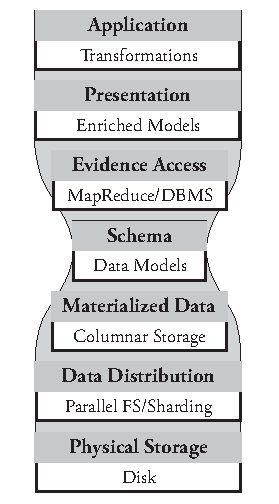
\includegraphics[width=0.6\linewidth]{stack-model.pdf}
\end{center}
\caption{A Stack Model for Scientific Computing}
\label{fig:stack-model}
\end{figure}

The seven layers of our stack model are decomposed as follows, traditionally numbered from bottom to
top:

\begin{enumerate}
\item {\bf Physical Storage:} This layer coordinates data writes to physical media.
\item {\bf Data Distribution:} This layer manages access, replication, and distribution of the files that have
been written to storage media.
\item {\bf Materialized Data:} This layer encodes the patterns for how data is encoded and stored. This
layer determines I/O bandwidth and compression.
\item {\bf Data Schema:} This layer specifies the representation of data, and forms the narrow waist of the
stack which separates access from execution.
\item {\bf Evidence Access:} This layer provides us with primitives for processing data, and allows us to
transform data into different views and traversals.
\item {\bf Presentation:} This layer enhances the data schema with convenience methods for performing
common tasks and accessing common derived fields from a single element.
\item {\bf Application:} At this level, we can use our evidence access and presentation layers to compose
the algorithms to perform our desired analysis.
\end{enumerate}

A well defined software stack has several other significant advantages. By limiting application
interactions with layers lower than the presentation layer, application developers are given a clear and
consistent view of the data they are processing, and this view of the data is independent of whether the
data is local or distributed across a cluster or cloud. By separating the API from the data access layer,
we improve flexibility. With careful design in the data format and data access layers, we can seamlessly
support conventional flat file access patterns, while also allowing easy access to data with database
methods. By treating the compute substrate and storage as separate layers, we also drastically increase
the portability of the APIs that we implement.

As we discuss in more detail in~\S\ref{sec:genomics-pipeline}, current scientific systems bleed functionality
between stack layers. An exemplar is the SAM/BAM and CRAM formats, which expect data to be sorted by
genomic coordinate. This modifies the layout of data on disk~(level 3, Materialized Data), which then
constrains how applications traverse datasets~(level 5, Evidence Access). Beyond constraining
applications, this leads to bugs in applications which are difficult to detect. To resolve this, we demonstrate
several ways to efficiently implement conventional scientific traversals
in~\S\ref{sec:optimizations-scientific-processing}. These traversals are implemented in the evidence access
layer, and are independent of anything below the schema.

The idea of decomposing scientific applications into a stack model is not new; Bafna et al~\cite{bafna13}
made a similar suggestion in 2013. We borrow some vocabulary from Bafna et al, but our approach is
differentiated in several critical ways:

\begin{itemize}
\item Bafna et al consider the stack model specifically in the context of data management systems for
genomics; as a result, they bake current methodologies into the stack. In our opinion, a good stack design
should serve to abstract layers from methodologies/implementations. If not, future technology trends may
obsolete a layer of the stack and render the stack irrelevant.
\item Bafna et al define a binary data format as the narrow waist in their stack, instead of a schema. While
these two seem interchangeable, they are not in practice. A schema is a higher level of abstraction and
allows for data serialization techniques to be changed as long as the same schema is still provided.
\item Notably, Bafna et al use this stack model to motivate GQL~\cite{kozanitis14}. While a query system
should provide a way to process and transform data, Bafna et al instead move this system down to the
data materialization layer. We feel that this inverts the semantics that a user of the system would prefer
and makes the system harder to use.
\end{itemize}

\section{Case Studies}
\label{sec:case-studies}

To validate our architectural choices, we have implemented pipelines for processing short read genomic
data and astronomy image processing. Both of these pipelines are implemented using
Spark~\cite{zaharia10}, Avro~\cite{avro}, and Parquet~\cite{parquet}. We have chosen these two
applications as they fit in different areas in the design space. 

\subsection{Genomics Pipeline}
\label{sec:genomics-pipeline}

Contemporary genomics has been revolutionized by ``next generation'' sequencing
technologies~(NGS), which have driven a precipitous drop in the cost of running genomic
assays~\cite{nhgri}. Although there are a variety of sequencing technologies in use, the majority of
sequence data comes from the Illumina/Solexa sequencing platform, which uses a
``sequencing-by-synthesis'' technique to generate \emph{short read} data~\cite{metzker09}, where a
sequencing run will generate many reads that are between 50 and 250 bases in length. In addition to
adjusting the length of the reads, we can control the amount of the data that is generated by
changing the amount of the genome that we sequence, or the amount of redundant sequencing that
we perform~(the average number of reads that covers each base, or \emph{coverage}). A single
human genome sequenced at 60$\times$ coverage will produce approximately 1.4 billion reads,
which is approximately 600 GB of raw data, or 225 GB of compressed data. For each read, we also
are provided \emph{quality scores}, which represent the likelihood that the base at a given position
was observed.

One of the most common genomic analyses is \emph{variant calling}, which is a statistical process to
infer the sites at which a single individual varies from the \emph{reference genome}.\footnote{The
reference genome represents the ``average'' genome for a species. The Human Genome
Project~\cite{lander01} assembled the first human reference genome.} This process consists of the
following general steps:

\begin{enumerate}
\item \textbf{Alignment:} For each read, we find the position in the genome that the read is most likely to
have come from. As an exact search is too expensive, there has been an extensive amount of research
which has focused on indexing strategies for improving alignment performance~\cite{li10, li11,
zaharia11}. This process is parallel per sequenced read.
\item \textbf{Pre-processing:} After reads have been aligned to the genome, we perform several
preprocessing steps to eliminate systemic errors in the reads. This may involve recalibrating the
observed quality scores for the bases, or locally optimizing the read alignments. We will present a
description of several of these algorithms in~\S\ref{sec:genomics-pipeline}; for a more detailed
discussion, we refer readers to DePristo et al~\cite{depristo11} and Massie et al~\cite{massie13}.
\item \textbf{Variant calling:} Variant calling is a statistical process which uses the read alignments
and the observed quality scores to compute whether a given sample \linebreak matches or diverges
from the reference genome. This process is typically parallel per position or region in the genome.
\item \textbf{Filtration:} After variants have been called, we want to filter out false positive variant calls.
We may perform queries to look for variants with borderline likelihoods, or we may look for clusters of
variants, which may indicate that a local error has occurred. This process may be parallel per position,
or may involve complex traversals of the genomic coordinate space.
\end{enumerate}

This process is very expensive to run; the current best practice pipeline uses the BWA tool~\cite{li10} for
alignment and the GATK~\cite{mckenna10, depristo11} for pre-processing, variant calling, and filtration.
Current benchmark suites have measured this pipeline as taking between 90 and 130 hours to run
end-to-end~\cite{talwalkar14}. Recent projects have achieved dramatic improvements in alignment and
variant calling performance~\cite{zaharia11, rimmer14}. Since this leaves the pre-processing stages as
the main performance bottleneck, we've chosen to focus on those stages. We have focused on
implementing the four most time consuming pre-processing stages, as well as \texttt{flagstat}, a
command which is used for quality control~(QC). In the remainder of this section, we describe the
stages that we have implemented, and the techniques we've used to improve performance and
accuracy. We omit detailed pseudocode here, but make pseudocode available in
Appendix~\ref{sec:genomics-pseudocode}.

\paragraph{Sorting}
\label{sec:sorting}
This phase sorts all reads by the position of the start of their alignment. The implementation of this
algorithm is trivial, as Spark provides a sort primitive~\cite{zaharia10}; we solely need to define an
ordering for genomic coordinates, which is well defined. In practice, an explicit sort is unnecessary when
using the rest of our MapReduce-based pipeline. We have included sort to enable the use of legacy
tools which require sorted input.

\paragraph{Duplicate Removal} 
\label{sec:duplicate-removal}
During the process of preparing DNA for sequencing, errors in the sample preparation and polymerase
chain reaction~(PCR) stages can cause the duplication of reads. Detection of duplicate reads requires
matching all reads by their position and orientation after read alignment. Reads with identical position
and orientation are assumed to be duplicates. When a group of duplicate reads is found, each read is
scored, and all but the top-scoring read are marked as duplicates.

We have validated our duplicate removal code against Picard~\cite{picard}, which is used by the GATK
for Marking Duplicates. Our implementation is fully concordant with the Picard/GATK duplicate removal
engine, with the exception of chimeric read pairs.\footnote{In a chimeric read pair, the two reads in the
read pairs align to different chromosomes; see Li et al~\cite{li10}.} Specifically, because Picard's
traversal engine is restricted to processing linearly sorted alignments, Picard mishandles these
alignments. Since our engine is not constrained by the underlying layout of data on disk, we are able
to properly handle chimeric read pairs.

\paragraph{Local Realignment} 
\label{sec:local-realignment}

In local realignment, we attempt to find areas where a variant allele causes reads to be locally misaligned
from the reference genome.\footnote{This is typically caused by the presence of insertion/deletion (INDEL)
variants; see DePristo et al~\cite{depristo11}.} In this algorithm, we first identify regions as targets for
realignment. In the GATK, this is done by traversing sorted read alignments. In our implementation, we
implement this as a fold over partitions where we generate targets, and then we merge the tree of targets.
This allows us to eliminate the data shuffle needed to achieve the sorted ordering. As part of this fold, we
must compute the convex hull of overlapping regions in parallel. We discuss this in more detail
in~\S\ref{sec:coordinate-system-joins}

After we have generated the targets, we associate reads to an overlapping target (if one exists). After
associating reads to realignment targets, we run the heuristic realignment algorithm which is described
in Appendix~\ref{sec:candidate-generation-realignment}.

\paragraph{Base Quality Score Recalibration~(BQSR)} 
\label{sec:bqsr}
During the sequencing process, systemic errors occur that lead to the incorrect assignment of base
quality scores. In this step, we label each base that we have sequenced with an \emph{error covariate}.
For each covariate, we count the total number of bases that we saw, as well as the total number of
bases within the covariate that do not match the reference genome. From this data, we apply a Yates'
correction to each covariate to recalculate the quality scores of all member bases:

\begin{equation}
\label{eqn:yates}
P_{err}^{cov} = \frac{\text{\# errors} \in cov + 1}{\text{\# observations} \in cov + 2}
\end{equation}

We have validated the concordance of our BQSR implementation against the GATK. The overall
differences are shown in Figure~\ref{fig:bqsr-concordance}\textbf{ (FIXME: Frank + Jey to update this
figure)}.  Across both tools, only 5000 of the $\sim$180B bases in the high-coverage NA12878 genome
dataset differ. After investigating this discrepancy, we have determined that this is due to an error in the
GATK, where paired-end reads are mishandled if the two reads in the pair overlap.

\begin{figure}[h]
\begin{center}
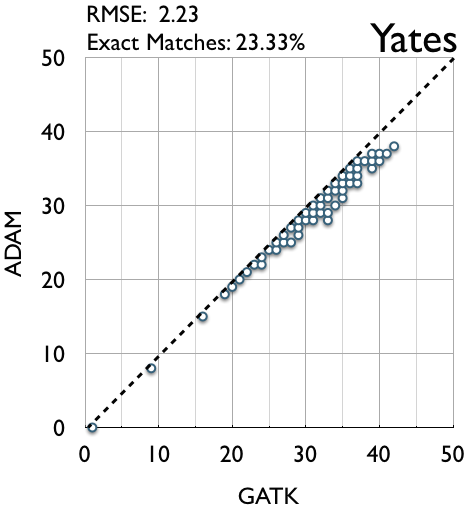
\includegraphics[width=0.9\linewidth]{graphs/bqsr-concordance.png}
\end{center}
\caption{BQSR Concordance vs. the GATK}
\label{fig:bqsr-concordance}
\end{figure}

For current implementations of these read processing steps, performance is limited by disk
bandwidth~\cite{diao15}. This bottleneck exists because the operations read in a SAM/BAM file, perform a
small amount of processing, and write the data to disk as a new SAM/BAM file. We achieve a performance
bump by performing our processing iteratively in memory. The four read processing stages can then be
chained together, eliminating three long writes to disk and an additional three long reads from disk.
Additionally, by rethinking the design of our algorithms, we are able to reduce overhead in several other
ways:

\begin{enumerate}
\item Current algorithms require the reference genome to be present on all nodes. This is then used to
look up the reference sequence that overlaps all reads. The reference genome is several gigabytes in size,
and performing a lookup in the reference genome can be costly due to its size. Instead, we leverage a field
in our schema to embed information about the reference in each read. This allows us to avoid broadcasting
the reference, and provides O(1) lookup.
\item Shared-memory genomics applications tend to be impacted significantly by false sharing of data
structures~\cite{zaharia11}. Instead of having data structures that are being written to in parallel, we
restructure our algorithms so that we only touch data structures from a single thread, and then merge
structures in a reduce phase. This has performance implications for the covariate calculation during
BQSR and the target generation phase of local realignment.
\item Without proper attention, the local realignment and duplicate marking tasks can suffer from bad
stragglers. This occurs due to a large amount of reads that either do not associate to a realignment target,
or that are unaligned. We pay special attention to these cases by manually randomizing the partitioning
for these reads. This resolves load imbalance and mitigates stragglers.
\item For the Flagstat command, we are able to project a limited subset of fields. Flagstat touches fewer
than 10 fields, which account for less than 3\% \textbf{(FIXME: Frank! check this number!)} of space on
disk. We discuss the performance implications of this further in~\S\ref{sec:column-store-perf}.
\end{enumerate}

\subsection{Astronomy Image Processing}
\label{sec:astronomy-image-processing}
The Montage~\cite{montage} application is a typical astronomy image processing pipeline that builds mosaics from small image 
tiles obtained from telescopes with the requirement of preserving the energy quantity and position for each pixel between the 
input and output images. The pipeline has multiple stages that can be grouped into the following phases.

\paragraph{Tile Reprojection}
The raw input images are reprojected with the defined scale as required in the final mosaic. 

\paragraph{Background Modeling}
This phase smoothes out the background levels between each pair of overlapped images and fits a plane to each of them. The phase can be further divided into steps of overlap calculation, difference image creation, and plane-fitting coefficient calculation.

\paragraph{Background Matching}
The background matching phase applies background removal to the reprojected images with the best solution derived from previous phase to smooth out the overlap regions.

\paragraph{Tile Mosaicing}
The tile masoning phase coadds all corrected images (after applying background matching to the reprojected images) into a aggregated mosaic file. This phase also involves a metadata processing stage before the mosaicing.

The tile reproduction, background modeling, and background matching phases are embarrassingly parallel, with each task (both computation and I/O) running independent from other tasks in the same phase. The tile mosaicing phase aligns the tiles of the matrix and applies a function (the function can be average, median, or count) to the overlapped pixels. All functions can be applied to the overlapped pixels in an embarrassingly parallel manner, while the I/O are done through a single process.

We care specifically about the tile mosaicing phase as the current implementation requires a preceding stage to summarize the metadata of all corrected images to produce a metadata table containing the tile positioning information. This particular stage has to read all input files into memory, but only accesses a small portion of the file. Also the current implementation parallelize the computation with each matrix row as the element, which results in inefficient input images replication when executed in a distributed environment. We address the first by explicitly declaring the image data schema and storing the images in a columnar store, so that all input images can be loaded to memory just once with all subsequent computation in memory. The metadata processing can access data that is continuous on a disk, while the rest of the I/O can be done in parallel.

\section{Data Access Optimizations for \\ Scientific Processing}
\label{sec:optimizations-scientific-processing}

\subsection{Coordinate System Joins}
\label{sec:coordinate-system-joins}

Genome informatics encompasses a wide array of experimental techniques and platforms, but almost all
of these methods share one characteristic in common: they produce datapoints which are tied to
locations in the genome through the use of genomic coordinates. The actual genome inside each cell is a
mammoth molecule, a collection of DNA polymers coated with (and wrapped around) proteins and
packed into the nucleus in a complex 3-dimensional shape. Bioinformaticians avoid this complexity by
representing all 3.2 billion bases of the human genome as a single long string (of A's, T', G's, and C's);
the ``tying'' of a datapoint or observation to the genome is represented by associating the data with a 1
dimensional point or interval. The reference genome defines a 1-dimensional coordinate space against
which all genomic phenomena are marked and measured.

A platform for scientific data processing in genomics needs to understand these 1-dimensional coordinate
systems because these become the basis on which data processing is parallelized. For example, when
calling variants from sequencing data, the sequence data which is localized to a single genomic region
(or ``locus'') can be processed independently from the data localized to a different region, as long as the
regions are far enough apart.

Not only parallelization, but many of the core algorithms and methods for data aggregation in genomics
are phrased in terms of geometric primitives on 1-D intervals and points: distance, overlap, and
containment.  An algorithm for calculating quality control metrics may try to calculate ``coverage,'' a count
of how many reads overlap each base in the genome. A method for filtering and annotating potential
variants might assess the validity of a variant by the quality and mapping characteristics of all reads
which overlap the putative variant.

In order to support these algorithms, we have implemented a ``region'' or ``spatial'' join  method, whose
outline in code is given below. The region join operation takes as input two sets (RDDs) of
\texttt{ReferenceRegions}, a data structure that represents intervals along the 1-D genomics coordinate
space. It produces, as output, the set of all \texttt{ReferenceRegion} pairs~(one from each of the two
input sets) such that the two regions overlap each other in terms of genomics spatial coordinates. 

\begin{lstlisting}
def partitionAndJoin[T, U](sc: SparkContext,
					 baseRDD: RDD[T],
					 joinedRDD: RDD[U])(implicit tMapping: ReferenceMapping[T],
					uMapping: ReferenceMapping[U],
					tManifest: ClassTag[T],
					uManifest: ClassTag[U]): RDD[(T, U)] = {

    val collectedLeft: Seq[(String, Iterable[ReferenceRegion])] =
      baseRDD
        .map(t => (tMapping.getReferenceName(t), 
			tMapping.getReferenceRegion(t))) 
        .groupBy(_._1) 
        .map(t => (t._1, t._2.map(_._2))) 
        .collect() 
        .toSeq 

    val multiNonOverlapping = 
	new MultiContigNonoverlappingRegions(collectedLeft)

    val regions = sc.broadcast(multiNonOverlapping)

    val smallerKeyed: RDD[(ReferenceRegion, T)] =
      baseRDD.keyBy(t => regions.value.regionsFor(t).head)

    val largerKeyed: RDD[(ReferenceRegion, U)] =
      joinedRDD.filter(regions.value.filter(_))
        .flatMap(t => regions.value.regionsFor(t)
			.map((r: ReferenceRegion) => (r, t)))

    val joined: RDD[(ReferenceRegion, (T, U))] =
      smallerKeyed.join(largerKeyed)

    val filtered: RDD[(ReferenceRegion, (T, U))] = 
	joined.filter({
	  case (rr: ReferenceRegion, (t: T, u: U)) =>
		tMapping.getReferenceRegion(t)
			.overlaps(uMapping.getReferenceRegion(u))
	})

    filtered.map(rrtu => rrtu._2)
  }
\end{lstlisting}

\subsection{Loading Remote Data}
\label{sec:loading-remote-data}

Another challenge faced by scientific systems is where to store the initial data files and how to load them
efficiently. Today, Spark is usually run in conjunction with the HDFS portion of the Hadoop stack---HDFS
provides data locality, access to local disk on each node of the Spark cluster, and robustness to node
failure. However, HDFS imposes significant constraints on running a Spark system in virtualized or
commodity computing (e.g. ``cloud'') environments.  It is easy to scale an HDFS-based system up to
larger numbers of nodes, but harder to remove nodes when the capacity is no longer needed.  

If we are willing to forgo the advantages of local disk and data locality provided by HDFS, however, we
may be able to relax some of these other restrictions and build a Spark-based cluster whose size is more
easily adjusted to the changing demands of the computation.  By storing our data in higher-latency,
durable, cheaper block storage (e.g. S3) we can also exploit the varying requirements of data
availability---not all datasets need to be kept ``hot'' in HDFS at all times, but can be accessed in a
piecemeal or parallelized manner through S3 interfaces.

Spark provides a particularly convenient abstraction for writing these new data access methods.  By
implementing our own data-loading RDD, we are able to allow a Spark cluster to access Parquet files
stored in S3 in parallel (each partition in the RDD reflects a row group in the corresponding Parquet file).
For Parquet files containing records that reflect known genomics datatypes (that are mapped to genomic
locations, for example) we generate simple index files for each Parquet file.  Each index file lists the
complete set of row groups for the Parquet file, as well which genomic regions contain data points within
each row group.  Our parallelized data loader reads this index file and restricts the partitions in the data
loading RDD it creates to only those Parquet row groups which possibly contain data relevant to the
user's query.

\section{Performance}
\label{sec:performance}


\subsection{Genomics Workloads}
\label{sec:genomics-performance}

\textbf{FIXME: These are old/outdated/need to be anonymized! Frank to update. Also, comment about data conversion cost.}

Table~\ref{tab:overview} previews the performance of ADAM for \textit{Sort}, \textit{Mark Duplicates},
and \textit{Flagstat}. The tests in this table are run on the high coverage \textit{NA12878} full genome
BAM file that is available from the 1000 Genomes project; the HG00096 low coverage BAM from 1000
Genomes is used later in this section\footnote{The files used for these experiments can be found on the
1000 Genomes ftp site, \url{ftp.1000genomes.ebi.ac.uk} in directory
\texttt{/vol1/ftp/data/NA12878/high\_coverage\_alignment/} for NA12878, and in directory
\texttt{/vol1/ftp/data/HG00096/alignment/} for HG00096.}. These tests have been run on the EC2 cloud,
using the instance types listed. We compute the cost of running each experiment by multiplying the
number of instances used by the total wall time for the run and by the cost of running a single instance
of that type for an hour, which is the process Amazon uses to charge customers.

\begin{table}[h]
\caption{\textit{Sort}, \textit{Mark Duplicates}, and \textit{Flagstat} Performance on NA12878}
\label{tab:overview}
\begin{tabular}{ l c c c c }
\hline
\multicolumn{5}{c}{\bf \textit{Sort}} \\
\bf Software & \bf EC2 profile & \bf Wall Time & \bf Speedup & \bf Cost \\
\hline
Picard 1.103 & 1 \texttt{hs1.8xlarge} & 17h 44m & 1$\times$ & \$81.57 \\
ADAM 0.5.0 & 1 \texttt{hs1.8xlarge} & 8h 56m & 2$\times$ & \$41.09 \\
ADAM 0.5.0 & 32 \texttt{cr1.8xlarge} & 33m & 32$\times$ & \$61.60 \\
ADAM 0.5.0 & 100 \texttt{m2.4xlarge} & 21m & 52$\times$ & \$56.00 \\ 
\hline
\multicolumn{5}{c}{\bf \textit{Mark Duplicates}} \\
\bf Software & \bf EC2 profile & \bf Wall Time & \bf Speedup & \bf Cost  \\
\hline
Picard 1.103 & 1 \texttt{hs1.8xlarge} & 20h 22m & 1$\times$ & \$93.68 \\
ADAM 0.5.0 & 100 \texttt{m2.4xlarge} & 29m & 42$\times$ & \$79.26 \\
\hline
\multicolumn{5}{c}{\bf \textit{Flagstat}} \\
\bf Software & \bf EC2 profile & \bf Wall Time & \bf Speedup & \bf Cost  \\
\hline
SAMtools 0.1.19 & 1 \texttt{hs1.8xlarge} & 25m 24s & 1$\times$ & \$1.95 \\
ADAM 0.5.0 & 32 \texttt{cr1.8xlarge} & 0m 46s & 33$\times$ & \$1.43 \\
\hline
\end{tabular}
\end{table}

Table~\ref{tab:machines} describes the instance types. Memory capacity is reported in Gibibytes~(GiB),
where 1 GiB is equal to $2^{30}$ bytes. Storage capacities are not reported in this table because disk
capacity does not impact performance, but the number and type of storage drives is reported because
aggregate disk bandwidth does impact performance. In our tests, the \texttt{hs1.8xlarge} instance is
chosen to represent a workstation. Network bandwidth is constant across all instances.

\begin{table}[h]
\caption{AWS Machine Types}
\label{tab:machines}
\begin{tabular}{ l c l }
\hline
\bf Machine & \bf Cost & \bf Description \\
\hline
\hline
\texttt{hs1.8xlarge} & \$4.60/hr/machine & 16 cores, 117GiB RAM, 24$\times$ HDD \\
\texttt{cr1.8xlarge} & \$3.50/hr/machine & 32 cores, 244GiB RAM, 2$\times$ SDD \\
\texttt{m2.4xlarge} & \$1.64/hr/machine & 8 cores, 68.4GiB RAM, 2$\times$ HDD \\
\hline
\end{tabular}
\end{table}

As can be seen from these results, the ADAM pipeline is approximately twice as fast as current pipelines
when running on a single node. Additionally, ADAM achieves speedup that is close to linear. This point is
not clear from Table~\ref{tab:overview}, as we change instance types when also changing the number of
instances used. To clarify, Figure~\ref{fig:speedup} presents speedup plots for the NA12878 high
coverage genome and the HG00096 low coverage genome~(16 GB BAM). These speedup
measurements are taken on a dedicated cluster of 82 machines where each machine has 24 Xeon
cores, 128GB of RAM, and 12 disks.

\begin{figure}[h]
\begin{center}
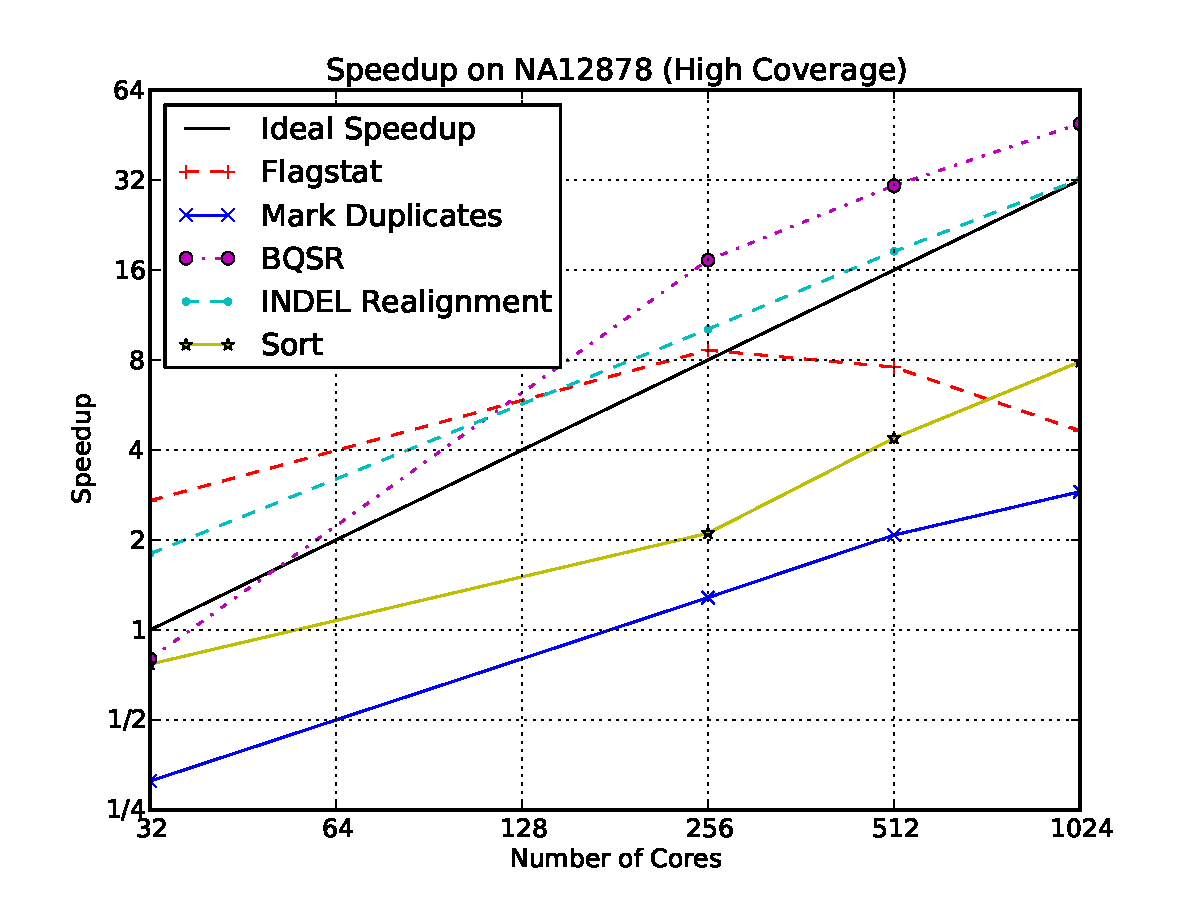
\includegraphics[width=0.99\linewidth]{graphs/speedup_na12878.pdf}
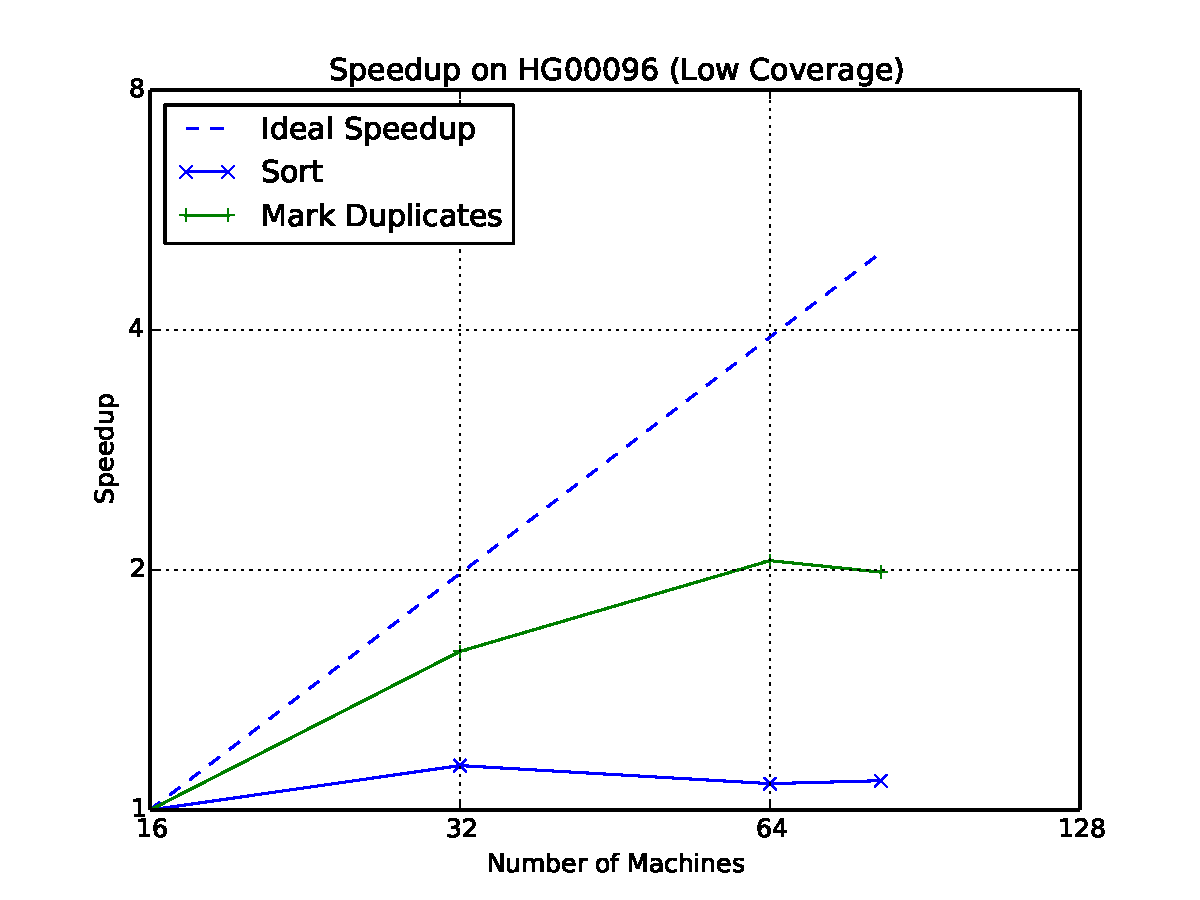
\includegraphics[width=0.99\linewidth]{graphs/speedup_hg00096.pdf}
\end{center}
\caption{Speedup when running \textit{Sort} and \textit{Mark Duplicates} on NA12878 and HG00096}
\label{fig:speedup}
\end{figure}

NA12878 sees linear speedup for both \textit{Sort} and \textit{Mark Duplicates} through 82 nodes. With
82 nodes, it takes 8.8 minutes to sort reads, and 14 minutes to mark duplicate reads across the 250GB
file. HG00096 is a significantly smaller genome at 16 GB. Although the speedup from sorting diminishes
after 16 nodes, duplicate marking sees speedup through 64 nodes. With HG00096 on 64 nodes, each
machine in the cluster is responsible for processing only 250MB of data. Sorting completes in 3.3
minutes, and duplicate marking completes in 2.3 minutes. The speedup is limited by several factors:

\begin{itemize}
\item Although columnar stores have very high read performance, they are limited by write performance.
Our tests exaggerate this penalty---as a variant calling pipeline will consume a large read file, but then
output a variant call file that is approximately two orders of magnitude smaller, the write penalty will be
reduced.
\item Additionally, for large clusters, straggler elimination is an issue. Phases of both \textit{Sort} and
\textit{MarkDuplicates} currently suffer from stragglers---we are in the process of addressing these
issues.
\end{itemize}

However, as noted above, speedup continues until we reach approximately 1GB of data per node for
sorting, or 250MB of data per node for duplicate marking. For a high coverage whole genome like
NA12878, this should theoretically allow speedup through 250 nodes for sorting and 1,000 nodes for
duplicate marking.

\subsection{Astronomy Workloads}
\label{sec:astro-workloads}

We use the 2MASS data and the Montage test case of 3x3 degree mosaicing with Galaxy m101 as the
center.  The tile mosaicing phase has 1.5~GB input data and produces a 1.2~GB aggregated output file.
We compare the SparkmAdd performance against the MPI based parallel implementation in Montage v3.3
(referred as MPImAdd in the following text). The performance is measured on 1, 4, and 16 Amazon
\texttt{m2.4xlarge} instances respectively. We use OrangeFS v2.8.8, a successor of PVFS~\cite{PVFS}, as
the shared file system across the instances to support MPImAdd. All eight cores on each instance are used
for both SparkmAdd and MPImAdd.

\begin{figure}[h]
\begin{center}
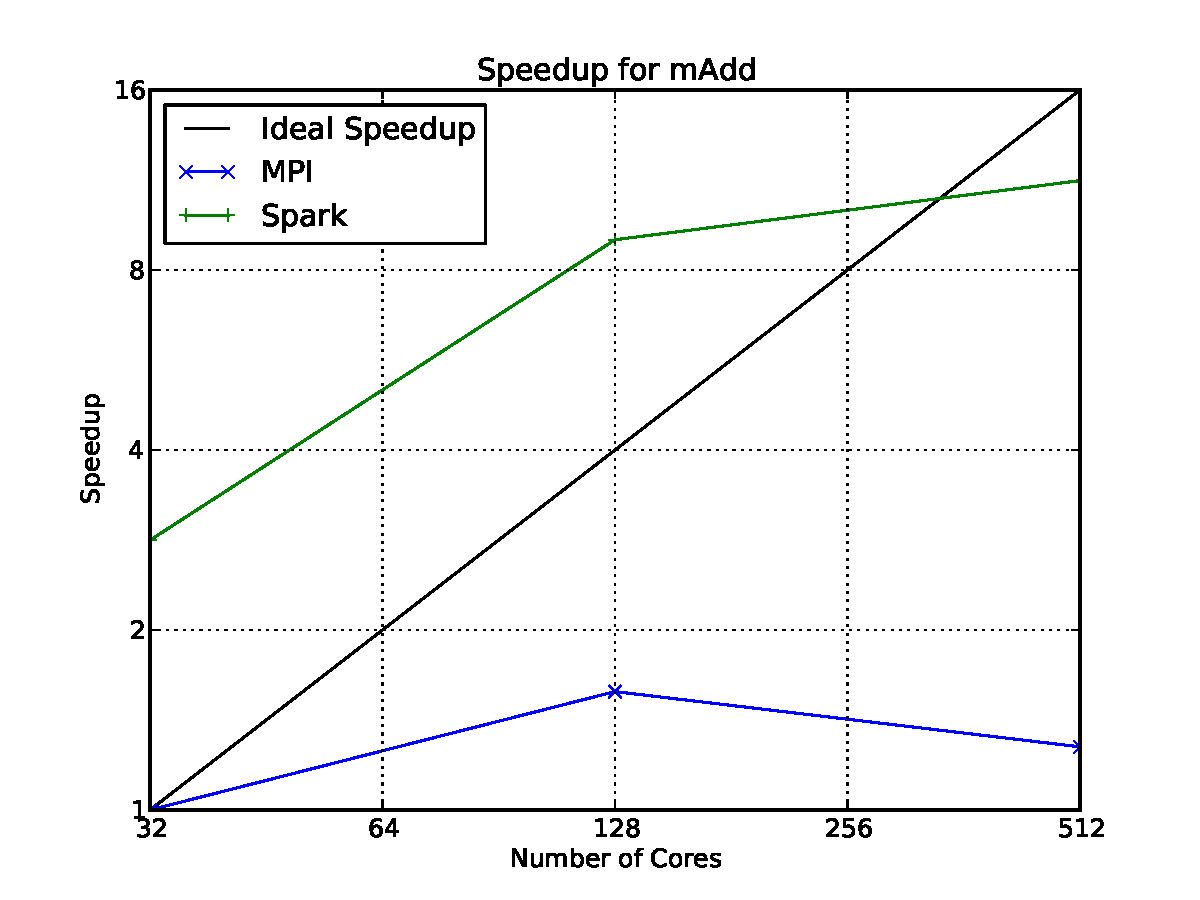
\includegraphics[width=0.99\linewidth]{graphs/speedup_madd.pdf}
\end{center}
\caption{Speedup when running \textit{mAdd} using MPI and Spark}
\label{fig:madd-speedup}
\end{figure}

As shown in Figure~\ref{fig:madd-speedup}, the SparkmAdd runs 1.3x, 2.8x, 3.3x faster than MPImAdd on
1, 4, and 16 instances with a data compression rate of 2.8x for input and 1.4x for output. The performance
improvement is contributed by multiple factors: less I/O amount, less I/O contention, and better data
locality. We manage to combine the metadata processing stage with mAdd together, since we explicitly
define the data schema in SparkmAdd, so that the same set of inputs can just be read once. We also
configure Parquet to compress the input and output data, so the actual I/O amount is reduced. Parquet
writes output files into HDFS in a contention free manner whereas MPI coordinates all processes to write to
a single file in the shared file system. The Spark framework lets the computation benefit from data locality,
while MPI distributes the computation across the available resources without concerning data placement.

\subsection{Column Store Performance}
\label{sec:column-store-perf}

\textbf{FIXME: This uses old data and also needs to be anonymized. Frank to fix. Also, discuss CRAM, and columnar representations for in-memory data.}

The decision to use a columnar store was based on the observation that most genomics applications are read-heavy. In this section,
we aim to quantify the improvements in read performance that we achieve by using a column store, and how far these gains can be
maximized through the use of projections.

\paragraph{Read Length and Quality:}
\label{sec:read-length-and-quality}

This microbenchmark scans all the reads in the file, and collects statistics about the length of the read, and the mapping quality score. Figure~\ref{fig:length-quality} shows
the results of this benchmark. Ideal speedup curves are plotted along with the speedup measurements. The speedups in this graph are plotted relative to the single machine Hadoop-BAM run.

\begin{figure}[h]
\begin{center}
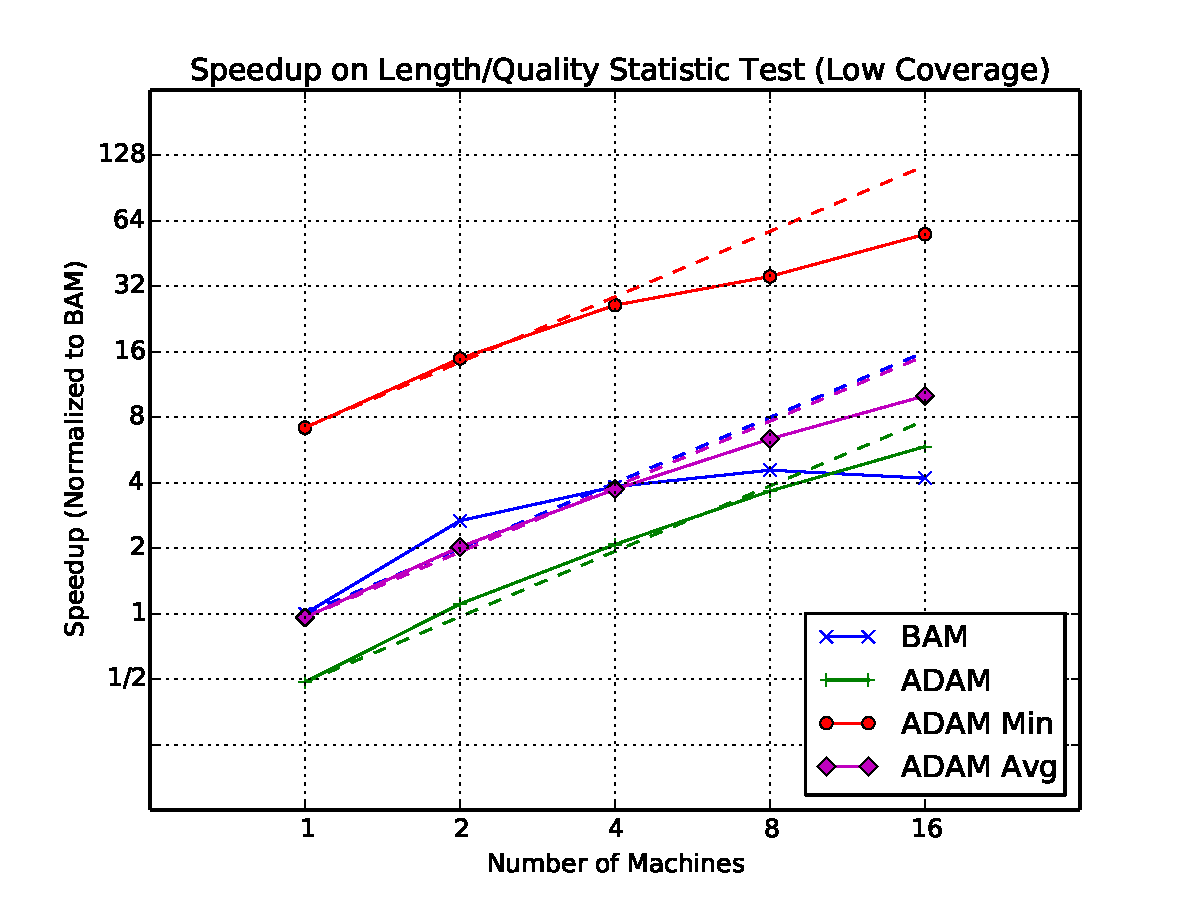
\includegraphics[width=\linewidth]{microbenchmarks/length_and_quality_low_coverage.pdf}
\end{center}
\caption{Read Length and Quality Speedup for HG00096}
\label{fig:length-quality}
\end{figure}

This benchmark demonstrates several things:

\begin{itemize}
\item ADAM demonstrates superior scalability over Hadoop-BAM. This performance is likely because ADAM files can be more evenly distributed across machines.
Hadoop-BAM must guess the proper partitioning when splitting files~\cite{niemenmaa12}. The Parquet file format that ADAM is based on is partitioned
evenly when it is written\cite{parquet}. This paritioning is critical for small files such as the one used in this test~---~in a 16 machine cluster, there is only 1 GB of
data per node, so imbalances on the order of the Hadoop file split size (128 MB) can lead to 40\% differences in loading between nodes.
\item Projections can significantly accelerate computation, if the calculation does not need all the data. By projecting the minimum dataset necessary
to calculate the target of this benchmark, we can accelerate the benchmark by $8\times$. Even a more modest projection leads to a $2\times$
improvement in performance.
\end{itemize}

\subsubsection{Predicate Pushdown}
\label{sec:predicate-pushdown}

Predicate pushdown is one of the significant advantages afforded to us through the use of Parquet	~\cite{parquet}. In traditional
pipelines, the full record is deserialized from disk, and the filter is implemented as a Map/Reduce processing stage. Parquet provides
us with predicate pushdown: we deserialize only the columns needed to identify whether the record should be fully deserialized. We
then process those fields; if they pass the predicate, we then deserialize the full record.

We can prove that this process requires no additional reads. Intuitively, this is true as the initial columns read would need to be read
if they were to be used in the filter later. However, this can be formalized. We provide a proof for this in Section C of the Appendix.
In this section, we seek to provide an intuition for how predicate pushdown can improve the performance of actual genomics workloads.
We apply predicate pushdown to implement read quality predication, mapping score predication, and predication by chromosome. 

\paragraph{Quality Flags Predicate:}
\label{sec:quality-flags-predicate}

This microbenchmark scans the reads in a file, and filters out reads that do not meet a specified quality threshold. We use the following
quality threshold:

\begin{itemize}
\item The read is mapped.
\item The read is at its primary alignment position.
\item The read did not fail vendor quality checks.
\item The read has not been marked as a duplicate.
\end{itemize}
This threshold is typically applied as one of the first operations in any read processing pipeline.

\paragraph{Gapped Predicate:}
\label{sec:gapped-predicate}

In many applications, the application seeks to look at a region of the genome~(e.g. a single chromosome or gene). We include this
predicate as a proxy: the gapped predicate looks for 1 out of every $n$ reads. This selectivity achieves performance analogous to filtering
on a single gene, but provides an upper bound as we pay a penalty due to our predicate hits being randomly distributed.

To validate the performance of predicate pushdown, we ran the predicates described above on the HG00096 genome on a
single AWS $m2.4xlarge$ instance. The goal of this was to determine the rough overhead of predicate projection.

Figure~\ref{fig:gapped-filter} shows performance for the gapped predicate sweeping $n$.

\begin{figure}[h]
\begin{center}
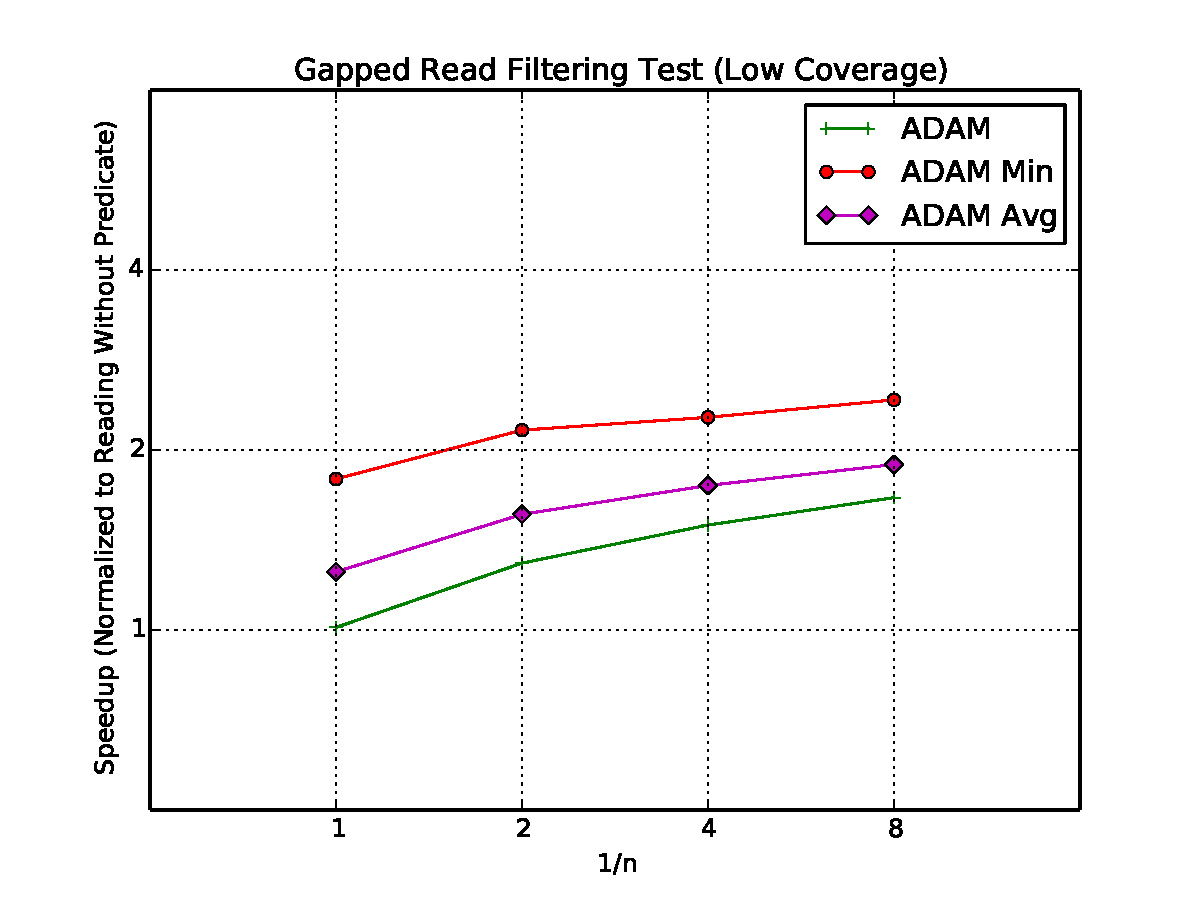
\includegraphics[width=\linewidth]{microbenchmarks/gapped_predicate_low_coverage.pdf}
\end{center}
\caption{Gapped Predicate on HG00096}
\label{fig:gapped-filter}
\end{figure}

There are several conclusions to be drawn from this experiment:

\begin{itemize}
\item As is demonstrated by equation~(\ref{eqn:predicate}) in Section C of the Appendix, we see the largest speedup when our predicate read set is significantly
smaller than our projection read set. For smaller projections, we see a fairly substantial reduction in speedup.
\item As the number of records that passes the predicate drops, the number of reads done to evaluate the predicate begins to become
a dominant term. This insight has one important implication: for applications that plan to access a very small segment of the data, accessing the
data as a flat file with a predicate is likely not the most efficient access pattern. Rather, if the predicate is regular, it is likely better to access
the data through a indexed database.
\end{itemize}

We additionally calculated the performance improvement that was achieved by using predicate pushdown instead of a Spark filter.
Table~\ref{tab:filter-vs-predicate} lists these results.

\begin{table}[h]
\caption{Predicate Pushdown Speedup vs. Filtering}
\label{tab:filter-vs-predicate}
\begin{center}
\begin{tabular}{| l | c  c c | c |}
\hline
\bf Predicate & \bf Min & \bf Avg & \bf Max & \bf Filtered \\
\hline
Locus & 1.19 & 1.17 & 0.94 & 3\% \\
Gapped, $n = 1$ & 1.0 & 1.0 & 1.01 & 0\% \\
Gapped, $n = 2$ & 1.22 & 1.27 & 1.29 & 50\% \\
Gapped, $n = 4$ & 1.31 & 1.42 & 1.49 & 75\% \\
Gapped, $n = 8$ & 1.37 & 1.58 & 1.67 & 87.5\% \\
\hline
\end{tabular}
\end{center}
\end{table}

These results are promising, as they indicate that predicate pushdown is faster than a Spark filter in most cases. We believe that the
only case that showed a slowdown (max projection on Locus predicate) is due to an issue in our test setup. We therefore can conclude
that filtering operations that can be performed statically at file load-in should be performed using predicate pushdown.

\section{Future Work}
\label{sec:future-work}

This work leverages columnar storage to improve performance and compression of data on disk,
with special emphasis on repetitive fields which can be run length encoded~(RLE). While this improves
disk performance, it has the side effect of making data consume significantly more space in memory
than on disk. We are currently investigating techniques that leverage the immutability of data in our
applications to reduce memory consumption. This may involve a pseudo-columnar data representation
in memory, or changes to Parquet and Avro's deserialization codec which would reuse allocated objects.

It is worth noting that there are many significant scientific applications (such as genome
assembly) that are expressed as traversal over graphs. Recent work by Simpson et al~(ABySS,
\cite{simpson09}) and Georganas et al~\cite{georganas14} has focused on using the Message Passing
Interface~(MPI) or Unified Parallel C~(UPC) to roll their own distributed graph traversal. Both systems
find that synchronization via message passing is a significant cost; specifically, the ABySS assembler
experiences scaling problems because it thrashes portions of the graph across nodes during traversal.
By building our system using Spark, we are able to leverage the GraphX processing library~\cite{xin13}.
We are in the process of developing a genome assembler using this library system, and believe that we
can achieve improved performance through careful graph partitioning. This involves algorithmic changes
to the graph creation and traversal phases to bypass ``knotted'' sections of the graph which
correspond to highly repetitive areas of the genome, which cause the major performance issues in MPI
based assemblers.

\section{Conclusion}
\label{sec:conclusion}

In this paper, we have advocated for a clean architecture for decomposing components in a scientific
system, and then demonstrated how to efficiently implement genomic and astronomy processing
pipelines using the open source Avro, Parquet, and Spark systems~\cite{avro, parquet, zaharia10}.
We demonstrate $>50\times$ performance improvements over conventional scientific processing
systems, along with linear strong scaling. Additionally, while an obvious advantage of using commodity
systems is code reuse, we've gained several valuable features for free:

\begin{enumerate}
\item Beyond efficient parallel performance, Parquet is also supported as a data format by several
database-like systems, like Spark-SQL and Impala. This allows us to support efficient database style
processing, without needing to manually retrofit a tool like GQL to the data~\cite{kozanitis14}.
\item While the native Spark Scala API provides rich programming abstractions, scientists may prefer
other language environments, like Python or R. Other scientific systems like SciDB~\cite{brown10}
support native Python and R bindings. Likewise, we provide distributed processing using Python
through PySpark.
\end{enumerate}

By rethinking the architecture of scientific data management systems, we have been able to achieve
significant scalability improvements while also expanding the methods which can be used to process
the data. The architecture we have developed is clean and principled and minimizes the
mixture-of-concerns which occurs in current scientific systems. Additionally, by applying our techniques
to both astronomy and genomics, we have demonstrated that the techniques are applicable to both
traditional matrix-based scientific computing, as well as novel scientific areas which have less structured
data.

\clearpage

\appendix

\bibliographystyle{abbrv}
\bibliography{adam} 

\section{Genomics Pseudocode}
\label{sec:genomics-pseudocode}

\textbf{FIXME: These are old/outdated/too long! Frank to rewrite.}

\subsection{Sort Implementation}
\label{sec:sort-implementation}

The ADAM Scala code for sorting a BAM file is succinct and relatively 
easy to follow. It is provided below for reference.

\begin{lstlisting}
def adamSortReadsByReferencePosition():
    RDD[ADAMRecord] = {
  rdd.map(p => {
    val referencePos = ReferencePosition(p) match {
      case None =>
        // Move unmapped reads to the end
        ReferencePosition(Int.MaxValue,
          Long.MaxValue)
      case Some(pos) => pos
    }
    (referencePos, p)
  }).sortByKey().map(p => p._2)
}
\end{lstlisting}

\subsection{BQSR Implementation}
\label{sec:bqsr-implementation}

Base Quality Score Recalibration is an important early data-normalization step in the bioinformatics pipeline, and after alignment
it is the next most costliest step. Since quality score recalibration can vastly improve the accuracy of variant calls~---~particularly for
pileup-based callers like the UnifiedGenotyper or Samtools mpileup. Because of this, it is likely to remain a part of bioinformatics pipelines.

BQSR is also an interesting algorithm in that it doesn't neatly fit into the framework of map reduce (the design philosophy of the GATK).
Instead it is an embarrassingly parallelizable aggregate. The ADAM implementation is:

\begin{lstlisting}
def computeTable(rdd: Records, dbsnp: Mask) :
  RecalTable = {
  
  rdd.aggregate(new RecalTable)(
    (table, read) => { table + read },
    (table, table) => { table ++ table })
}
\end{lstlisting}

The ADAM implementation of BQSR utilizes the MD field to identify bases in the read that mismatch the reference. This enables
base quality score recalibration to be entirely reference-free, avoiding the need to have a central Fasta store for the human
reference. However, dbSNP is still needed to mask out positions that are polymorphic (otherwise errors due to real variation will
severely bias the error rate estimates).

\subsection{Indel Realignment\\Implementation}
\label{sec:indel-realignment-implementation}

Indel realignment is implemented as a two step process. In the first step, we identify regions that have evidence of an insertion or
deletion. After these regions are identified, we generate candidate haplotypes, and realign reads to minimize the overall quantity
of mismatches in the region. The quality of mismatches near an indel serves as a good proxy for the local quality of an alignment.
This is due to the nature of indel alignment errors: when an indel is misaligned, this causes a temporary shift in the read sequence
against the reference sequence. This shift manifests as a run of several bases with mismatches due to their incorrect alignment.

\subsubsection{Realignment Target Identification}
\label{sec:realignment-target-identification}

Realignment target identification is done by converting our reads into reference oriented ``rods''\footnote{Also known as pileups: a
group of bases that are all aligned to a specific locus on the reference.}. At each locus where there is evidence of an insertion or a
deletion, we create a \emph{target} marker. We also create a target if there is evidence of a mismatch. These targets contain the indel
range or mismatch positions on the reference, and the range on the reference covered by reads that overlap these sites.

After an initial set of targets are placed, we merge targets together. This is necessary, as during the read realignment process, all
reads can only be realigned once. This necessitates that all reads are members of either one or zero realignment targets. Practically,
this means that over the set of all realignment targets, no two targets overlap.

The core of our target identification algorithm can be found below.

\begin{lstlisting}
def findTargets (reads: RDD[ADAMRecord]):
    TreeSet[IndelRealignmentTarget] = {

  // convert reads to rods
  val processor = new Read2PileupProcessor
  val rods: RDD[Seq[ADAMPileup]] = reads.flatMap(
      processor.readToPileups(_))
    .groupBy(_.getPosition).map(_._2)

  // map and merge targets
  val targetSet = rods.map(
      IndelRealignmentTarget(_))
    .filter(!_.isEmpty)
    .keyBy(_.getReadRange.start)
    .sortByKey()
    .map(new TreeSet()(TargetOrdering) + _._2)
    .fold(new TreeSet()(TargetOrdering))(
      joinTargets)

  targetSet
}
\end{lstlisting}

To generate the initial unmerged set of targets, we rely on the ADAM toolkit's pileup generation utilities~(see~\-S\ref{sec:reference-oriented-storage}).
We generate realignment targets for all pileups, even if they do not have indel or mismatch evidence. We eliminate pileups that do not contain indels
or mismatches with a filtering stage that eliminates empty targets. To merge overlapping targets, we map all of the targets into a sorted set. This set
is implemented using Red-Black trees. This allows for efficient merges, which are implemented with the tail-call recursive \emph{joinTargets} function:

\begin{lstlisting}
@tailrec def joinTargets (                                                                                                                                                               
  first: TreeSet[IndelRealignmentTarget],                                                                                                                                                                
  second: TreeSet[IndelRealignmentTarget]):
    TreeSet[IndelRealignmentTarget] = {

  if (!TargetOrdering.overlap(first.last,
      second.head)) {
    first.union(second)
  } else {
    joinTargets (first - first.last +
      first.last.merge(second.head),
      second - second.head)
  }
}
\end{lstlisting}

As we are performing a fold on an RDD which is sorted by the starting position of the target on the reference sequence, we know a priori that the elements
in the ``first'' set will always be ordered earlier relative to the elements in the ``second'' set. However, there can still be overlap between the two sets, as this
ordering does not account for the end positions of the targets. If there is overlap between the last target in the ``first'' set and the first target in the ``second''
set, we merge these two elements, and try to merge the two sets again.

\subsubsection{Candidate Generation\\and Realignment}
\label{sec:candidate-generation-realignment}

Candidate generation is a several step process:

\begin{enumerate}
\item Realignment targets must ``collect'' the reads that they contain.
\item For each realignment group, we must generate a new set of candidate haplotype alignments.
\item Then, these candidate alignments must be tested and compared to the current reference haplotype.
\item If a candidate haplotype is sufficiently better than the reference, reads are realigned.
\end{enumerate}

The mapping of reads to realignment targets is done through a tail recursive function that performs a binary search across the sorted set of indel alignment targets:

\begin{lstlisting}
@tailrec def mapToTarget (read: ADAMRecord,                                                                                                                                                        
  targets: TreeSet[IndelRealignmentTarget]):
    IndelRealignmentTarget = {

  if (targets.size == 1) {
    if (TargetOrdering.equals (targets.head, read)) {
      targets.head
    } else {
      IndelRealignmentTarget.emptyTarget
    }
  } else {
    val (head, tail) = targets.splitAt(
      targets.size / 2)
    val reducedSet = if (TargetOrdering.lt(
        tail.head, read)) {
      head
    } else {
      tail
    }
    mapToTarget (read, reducedSet)
  }
}
\end{lstlisting}

This function is applied as a groupBy against all reads. This means that the function is mapped to the RDD that contains all reads. A new RDD is generated where all
reads that returned the same indel realignment target are grouped together into a list.

Once all reads are grouped, we identify new candidate alignments. However, before we do this, we left align all indels. For many reads that show evidence of a single
indel, this can eliminate mismatches that occur after the indel. This involves shifting the indel location to the ``left''\footnote{To a lower position against the reference
sequence.} by the length of the indel. After this, if the read still shows mismatches, we generate a new consensus alignment. This is done with the
\emph{generateAlternateConsensus} function, which distills the indel evidence out from the read.

\begin{lstlisting}
def generateAlternateConsensus (sequence: String,
  start: Long, cigar: Cigar): Option[Consensus] = {
  var readPos = 0
  var referencePos = start

  if (cigar.getCigarElements.filter(elem =>
        elem.getOperator == CigarOperator.I ||
        elem.getOperator == CigarOperator.D
      ).length == 1) {
    cigar.getCigarElements.foreach(cigarElement =>
      { cigarElement.getOperator match {
        case CigarOperator.I => return Some(
          new Consensus(sequence.substring(readPos,
            readPos + cigarElement.getLength),
            referencePos to referencePos))
        case CigarOperator.D => return Some(
          new Consensus("",
          referencePos until (referencePos +
            cigarElement.getLength)))
        case _ => {
          if (cigarElement.getOperator
                .consumesReadBases &&
              cigarElement.getOperator
                .consumesReferenceBases
              ) {
            readPos += cigarElement.getLength
            referencePos += cigarElement.getLength
          } else {
            return None
          }
        }
      }
    })
    None
  } else {
    None
  }
}
\end{lstlisting}

From these consensuses, we generate new haplotypes by inserting the indel consensus into the reference sequence. The quality of each haplotype is measured
by sliding each read across the new haplotype, using \emph{mismatch quality}. Mismatch quality is defined for a given alignment by the sum of the quality scores
of all bases that mismatch against the current alignment. While sliding each read across the new haplotype, we aggregate the mismatch quality scores. We take
the minimum of all of these scores and the mismatch quality of the original alignment. This sweep is performed using the \emph{sweepReadOverReferenceForQuality}
function:

\begin{lstlisting}
def sweepReadOverReferenceForQuality (
    read: String,reference: String,
    qualities: Seq[Int]): (Int, Int) = {
  var qualityScores = List[(Int, Int)]()

  for (i <- 0 until (reference.length -
      read.length)) {
    qualityScores = (
      sumMismatchQualityIgnoreCigar(
        read,
        reference.substring(i, i + read.length),
          qualities),
        i) :: qualityScores
  }

  qualityScores.reduce ((p1: (Int, Int),
      p2: (Int, Int)) => {
    if (p1._1 < p2._1) {
      p1
    } else {
      p2
    }
  })
}
\end{lstlisting}

If the consensus with the lowest mismatch quality score has a log-odds ratio~(LOD) that is greater than $5.0$ with respect to the reference, we realign the reads.
This is done by recomputing the cigar and MDTag for each new alignment. Realigned reads have their mapping quality score increased by 10 in the Phred scale.

\subsection{Duplicate Marking\\Implementation}
\label{sec:duplicate-marking-implementation}

The following ADAM code, reformatted for this report, expresses the algorithm succinctly in 42 lines of Scala code.

\begin{lstlisting}
for (((leftPos, library), readsByLeftPos) <- 
    rdd.adamSingleReadBuckets()
       .keyBy(ReferencePositionPair(_))
       .groupBy(leftPositionAndLibrary);

buckets <- {

leftPos match {
 // These are all unmapped reads. 
 // There is no way to determine if
 // they are duplicates
 case None =>
    markReads(readsByLeftPos.unzip._2,
      areDups = false)
 // These reads have their left position mapped
 case Some(leftPosWithOrientation) =>
   // Group the reads by their right position
   val readsByRightPos = readsByLeftPos.groupBy(
     rightPosition)
   // Find any reads with no right position
   val fragments = readsByRightPos.get(None)
   // Check if we have any pairs
   // (reads with a right position)
   val hasPairs = readsByRightPos.keys
     .exists(_.isDefined)
   if (hasPairs) {
     // Since we have pairs,
     // mark all fragments as duplicates
     val processedFrags = if (fragments.isDefined
     ) {
       markReads(fragments.get.unzip._2,
         areDups = true)
     } else {
       Seq.empty
     }
     val processedPairs = 
         for (buckets <- (readsByRightPos - None)
           .values;
             processedPair <- 
                scoreAndMarkReads(buckets.unzip._2)) 
        yield processedPair
     processedPairs ++ processedFrags
   } else if (fragments.isDefined) {
     // No pairs. Score the fragments.
     scoreAndMarkReads(fragments.get.unzip._2)
   } else {
     Seq.empty
   }
};
read <- buckets.allReads) yield read
\end{lstlisting}

For lines 1-4, all reads with the same record group name and read name are collected 
into buckets. These buckets contain the read and optional mate or secondary alignments.
Each read bucket is then keyed by 5 $'$ position and orientation and grouped together by
left (lowest coordinate) position, orientation and library name.

For lines 8-41, we processed each read bucket with a common left 5$'$ position. Unmapped
reads are never marked duplicate as their position is not known. Mapped reads with a common
left position are separated into paired reads and fragments. Fragments, in this context,
are reads that have no mate or should have a mate but it doesn't exist.

If there are pairs in a group, all fragments are marked duplicates and the paired reads are grouped
by their right 5$'$ position. All paired reads that have a common right and left 5$'$
position are scored and all but the highest scoring read is marked a duplicate.

If there are no pairs in a group, all fragments are scored and all but the highest scoring fragment
are marked duplicates.

%\balancecolumns
% That's all folks!
\end{document}
